\ifdefined\included
\else
\documentclass[a4paper,11pt,twoside]{StyleThese}
\include{formatAndDefs}
\sloppy
\begin{document}
\setcounter{chapter}{0} %% Numéro du chapitre précédent ;)
\dominitoc
\faketableofcontents
\fi

\chapter{Background \& State-of-the-art}
\minitoc

\section{Cloud-Edge Continuum}

The evolution of computing infrastructures has been marked by a shift from centralized Cloud architectures to a more distributed and dynamic model that integrates the strengths of Cloud computing. While Cloud computing revolutionized the way we store, process, and access data, by providing scalability and flexibility to users, it remains limited on latency, network bottlenecks, or privacy. Edge computing was introduced for applications that requires real-time responsiveness, bringing computation closer to data sources, reducing latency and enabling faster, more efficient processing for time-sensitive tasks.

This transition from Cloud-centric architectures to Edge-enabled architectures has led to the Cloud-Edge continuum \cite{khalyeyevCharacterizationEdgeCloudContinuum2023}, an hybrid framework that makes use of the best of both worlds. By distributing workloads between centralized Cloud resources and decentralized Edge nodes, this continuum increases performance, while decreasing latency. It supports innovative use cases, from autonomous IoT systems and smart cities, to industrial automation and immersive technologies.

\subsection{Service orchestration in the Cloud-Edge Continuum}

At the heart of modern computing lies the concept of \emph{services}. To fully exploit the potential of these services, \emph{service orchestration} emerges as the strategic approach for automating and coordinating these services, across Cloud and Edge infrastructures.

\subsubsection{Definition of a service}

In computing, a \emph{service} refers to a self-contained, modular component or set of components, that performs a specific function (or multiple), to support other software, applications, or end-users. Services are designed to be reusable, scalable, and often operate independently of the underlying infrastructure.

In our context, \emph{service} is used as generic term that can refer to a wide range of entities, such as:

\begin{itemize}
    \item A discrete \emph{task} (e.g. data processing)
    \item A standalone \emph{application} (e.g. web server, database)
    \item A \emph{microservice} in a container
    \item Or any other functional unit that provides value to users or other systems.
\end{itemize}

Services are often deployed and managed using Cloud-native technologies, such as virtualization and containerization. These approaches make services more portable, more resource efficient, and more isolated, allowing them to run consistently across diverse environments. A deeper examination of these technologies is provided in Section \ref{sec:cloud-native}.

\subsubsection{What is service orchestration?}

Service orchestration involves the strategic allocation of resources and deployment of services in a computing environment. Its key aspects include:

\begin{itemize}
    \item \emph{Resource management}: Provisioning, configuring, and scaling resources to meet application or workload demands.
    \item \emph{Coordination}: Ensuring harmonious collaboration among services to achieve desired outcomes.
    \item \emph{Lifecycle automation}: Automating the entire lifecycle of services and resources, by reducing manual intervention and streamlining repetitive tasks.
    \item \emph{Efficiency and optimization}: Intelligent resource allocation, efficient workflows, and automated deployments to reduce operational costs.
    \item \emph{Adaptability}: Dynamically adjusting to changing conditions, such as fluctuating workloads, system failures, or evolving requirements, to maintain responsiveness and robustness. 
\end{itemize}

This adaptability is particularly critical in modern computing environments, where services are increasingly distributed across the Edge. By extending orchestration capabilities from centralized Cloud infrastructures to Edge devices, organizations can achieve lower latency, improved scalability, and enhanced real-time processing, key requirements for applications like IoT, AI, and distributed analytics.

\subsection{Cloud-Native technologies} \label{sec:cloud-native}

Virtualization and containerization are fundamental technologies that have reshaped modern computing, particularly in Cloud computing. Together, these technologies empower it to deliver scalability, resilience, and agility. They enable quick application deployment, efficient resource management, and support for advanced models like serverless computing or container orchestration (e.g., Kubernetes \cite{Kubernetes2026}).

\subsubsection{Virtualization}

Virtualization enables the execution of multiple VMs\nomenclature{VM}{Virtual Machine} on a single physical host, where each VM includes its own guest OS\nomenclature{OS}{Operating System}, kernel, and virtualized hardware resources such as CPU, memory, and storage \cite{rodriguez-haroSummaryVirtualizationTechniques2012}. This abstraction is provided by a hypervisor (e.g., VMware, KVM, or Hyper-V), which enforces strong hardware-level isolation between VMs. While this isolation provides security and resource allocation, it also introduces significant overhead in terms of resource consumption, VM image size, and startup time. Virtualization was widely popularized with the emergence of Cloud computing, as it allows Cloud providers to efficiently multiplex physical infrastructure among multiple tenants while ensuring isolation, flexibility, and on-demand resource provisioning.

\subsubsection{Containerization}

Containerization emerged as a lightweight alternative to traditional virtualization in response to the increasing overhead and limited agility of virtual machines, particularly for large-scale, dynamic applications \cite{watadaEmergingTrendsTechniques2019}. Instead of virtualizing hardware, containerization relies on OS-level virtualization, where applications are packaged with their dependencies and executed in isolated containers that share the host operating system kernel. This design significantly reduces resource overhead, image size, and startup time, enabling higher workload density and faster scaling compared to VMs. Table \ref{tab:diff_virt_cont} shows the differences between virtualization and containerization. Containerization was popularized in modern Cloud-native architectures, especially for microservices and continuous deployment workflows, with orchestration platforms such as Kubernetes \cite{Kubernetes2026} providing automated deployment and scaling. The same principles that motivated container adoption in Cloud environments, also make containerization, and more generally Cloud technologies, highly suitable for Edge computing. At the Edge, where resources are more constrained, heterogeneous, and geographically distributed, containers and lightweight virtualized workloads enable flexible service placement, mobility, and isolation, allowing Cloud applications to be effectively extended and adapted to Edge infrastructures.


\begin{table}[!h]
    \centering
    \begin{tabular}{|>{\centering\arraybackslash}p{0.2\linewidth}|>{\centering\arraybackslash}p{0.35\linewidth}|>{\centering\arraybackslash}p{0.35\linewidth}|}
        \hline
         &  Virtualization& Containerization\\
         \hline \hline
         Size& Large (includes guest OS) & Small (only libraries)\\
         \hline
         Isolation&  Hardware-level& OS-level\\
         \hline
         Kernel&  Own kernel& Shared kernel\\
         \hline
         Startup time&  Slower& Faster\\
         \hline
         Resource allocation&  Stricter with higher minimum requirements& More flexible with lower requirements\\
         \hline
         Flexibility&  Heterogeneous OS kernels& Requires same OS kernel\\
         \hline
    \end{tabular}
    \caption{Differences between virtualization and containerization.}
    \label{tab:diff_virt_cont}
\end{table}

\subsection{Edge Computing}

In recent years, the Edge computing paradigm has gained significant attention due to its ability to process data closer to the data source, thereby reducing end-to-end latency, bandwidth consumption, and dependence on centralized infrastructures \cite{caoOverviewEdgeComputing2020}. This paradigm represents a fundamental shift from traditional Cloud computing, where data processing and storage are primarily performed in large, centralized data centers often located far from end users. While Cloud computing offers large computational resources and scalability, it can suffer from increased latency, network congestion, and privacy concerns for delay-sensitive or data-intensive applications. Edge computing addresses these limitations by decentralizing computation and enabling localized processing at the network edge, closer to users and devices.

Edge computing is also tightly coupled with the IoT\nomenclature{IoT}{Internet of Things}, as IoT systems generate massive volumes of data from geographically distributed, resource-constrained devices such as sensors, actuators, and smart objects. Processing all this data in the Cloud is often impractical, so, by offloading computation to Edge nodes located near IoT devices, Edge computing enables real-time analysis, faster decision-making, improved reliability, and reduced communication overhead. Consequently, Edge computing is widely regarded as a key enabler for large-scale IoT deployments and latency-critical applications.

A commonly adopted architectural representation of Edge computing is the three-layer model \cite{kongEdgeComputingInternet2022}, illustrated in Fig. \ref{fig:3_layer_model}, which typically consists of the device layer, the Edge layer, and the Cloud layer, each responsible for different levels of data generation, processing, and storage.

\begin{figure}[!h]
    \centering
    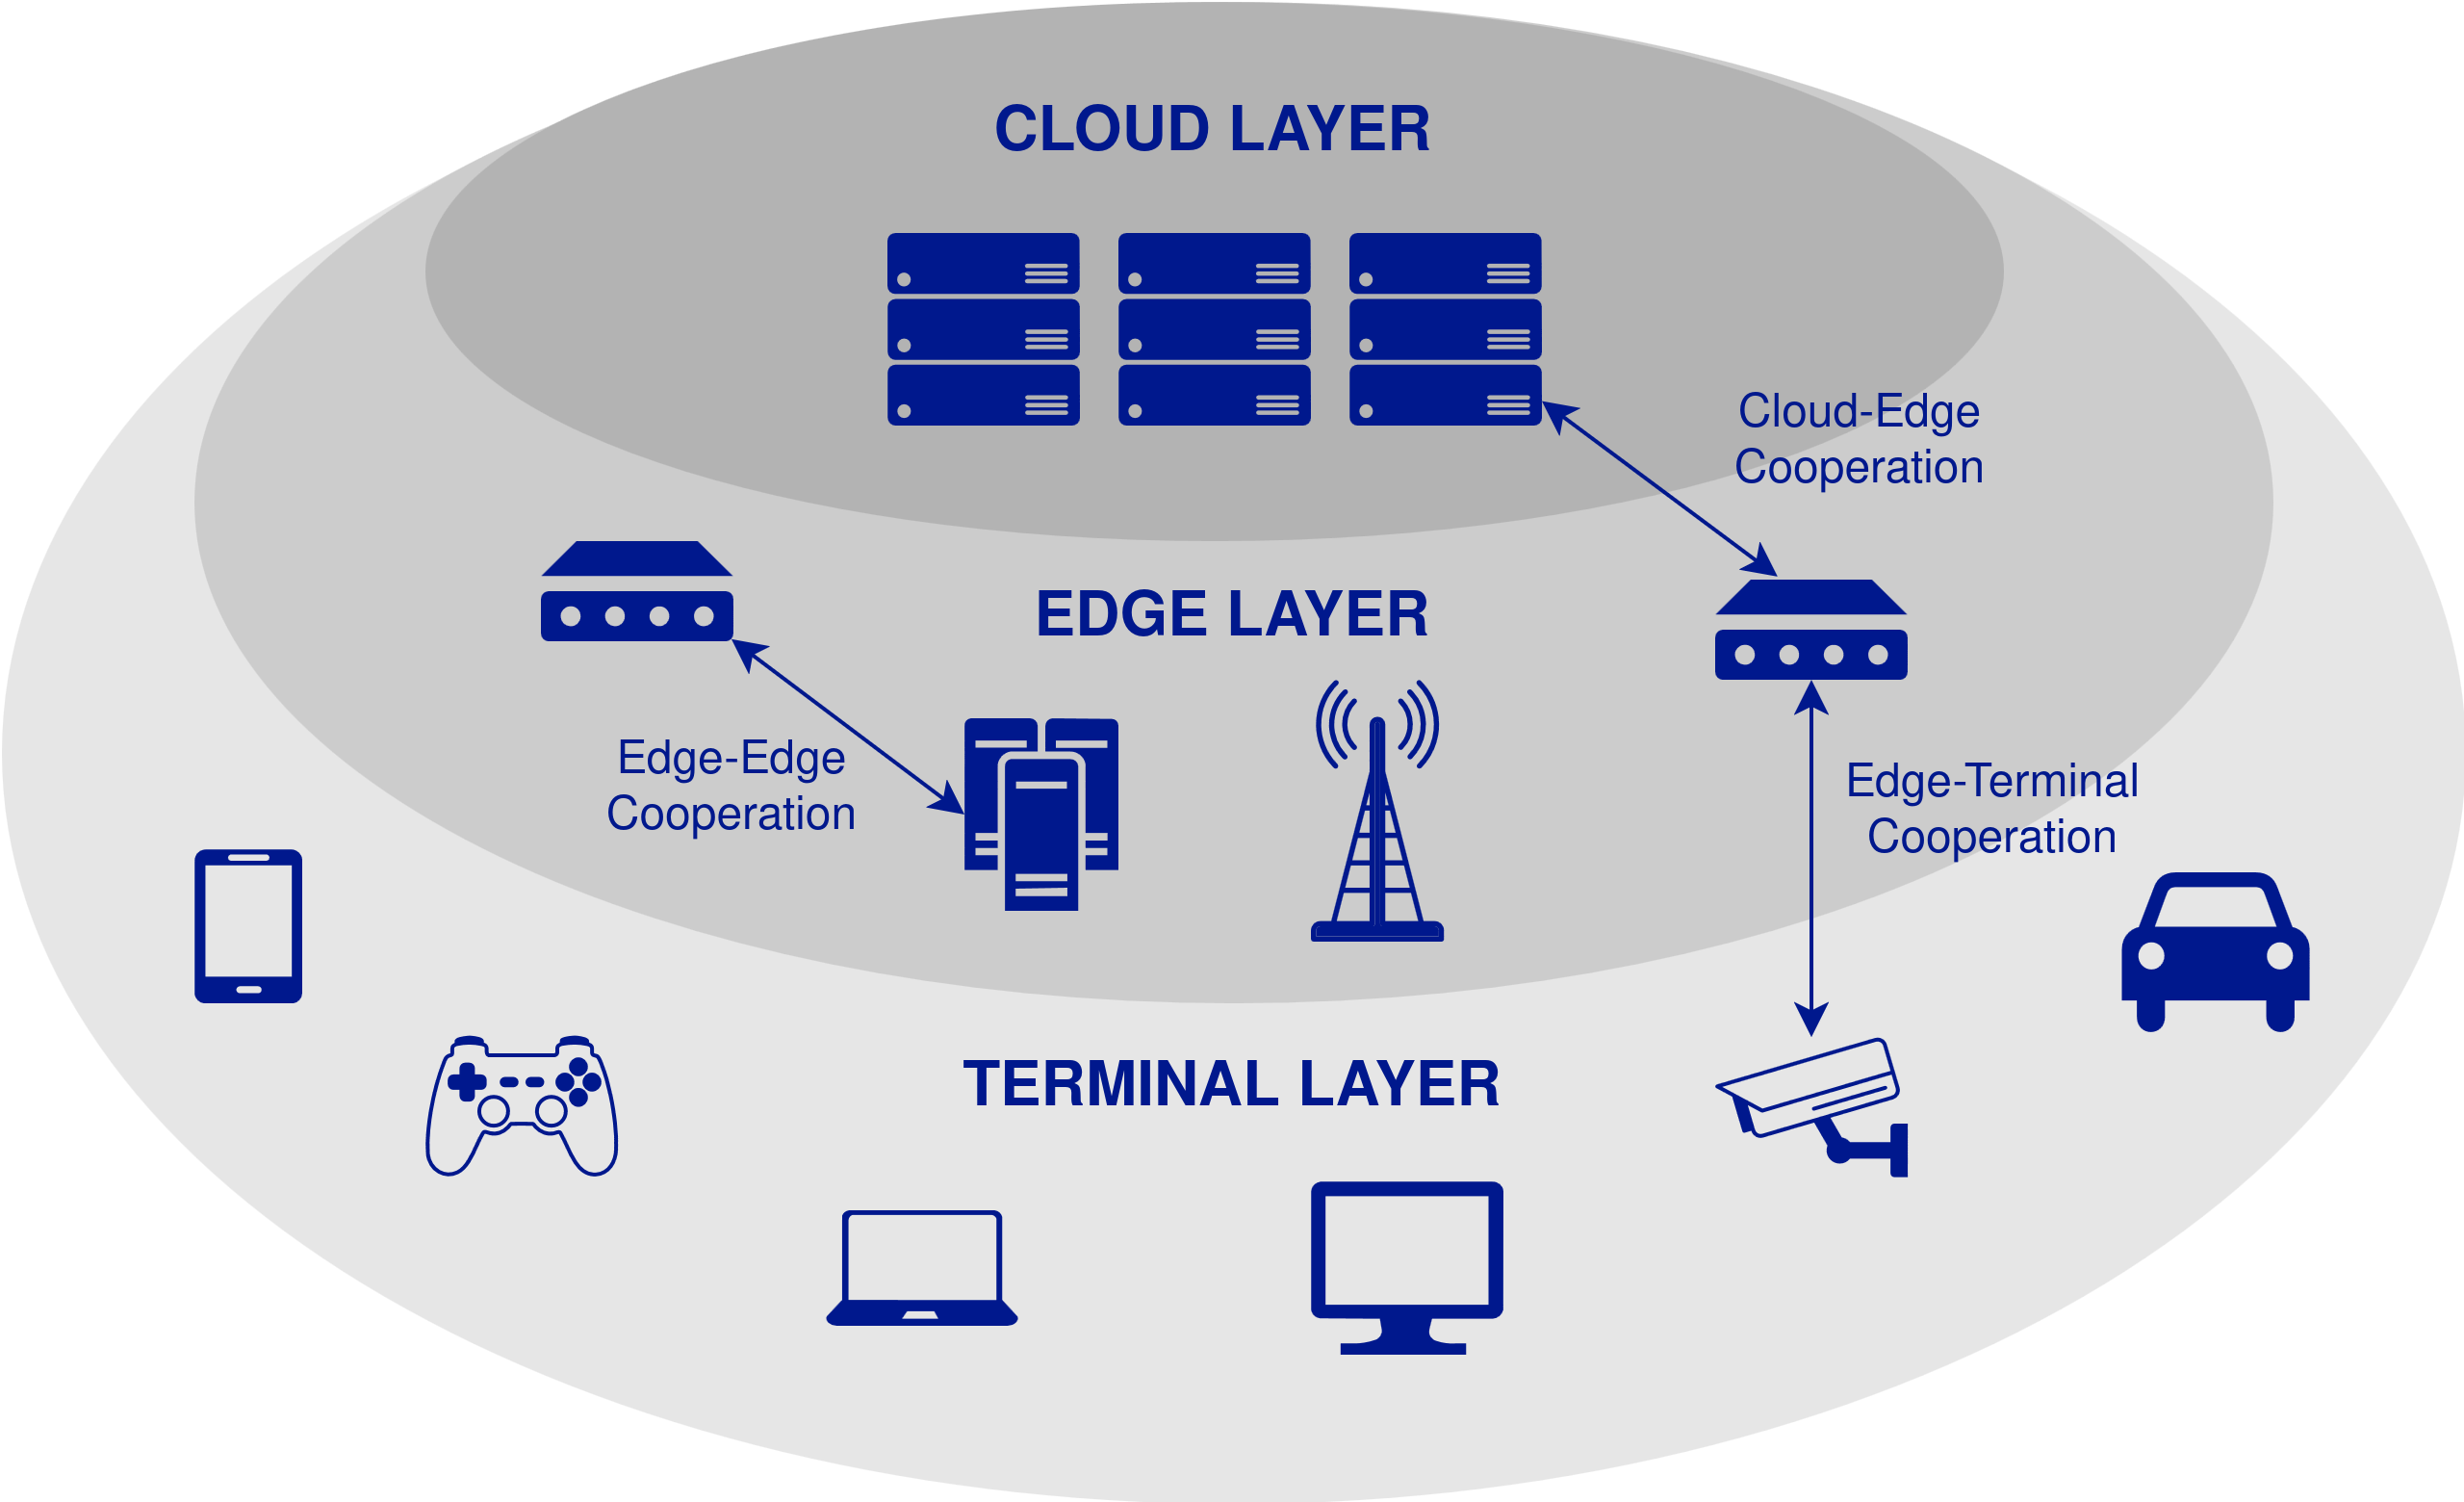
\includegraphics[width=0.8\linewidth]{figures/chapter1/3_layer_model.png}
    \caption{Three-layer model for representing Edge computing.}
    \label{fig:3_layer_model}
\end{figure}

Smarter service orchestration techniques are required to efficiently manage and allocate resources across geographically distributed Edge nodes, where heterogeneity, limited capacity, and dynamic workloads pose significant challenges. In such environments, energy efficiency becomes a critical concern, as Edge devices often operate under strict power constraints and may be deployed in locations with limited access to stable energy supplies. Consequently, service orchestration mechanisms must explicitly account for energy consumption, aiming to minimize power usage while preserving application performance and QoS\nomenclature{QoS}{Quality-of-Service}.

In parallel, the integration of renewable energy sources into Edge computing infrastructures has gained increasing attention as a means to improve the sustainability of Edge service provisioning. Edge nodes may be partially or fully powered by renewable sources such as solar or wind energy, often complemented by local energy storage systems (e.g., batteries) to mitigate the intermittency of energy generation. This introduces a new dimension to the orchestration problem, as decisions must consider not only computational and networking resources, but also the availability of harvested energy, battery state of charge, and energy forecasting. Energy-aware and renewable-aware orchestration strategies can use this data to shift workloads in space or time, prioritize nodes with a surplus of green energy, and reduce reliance on grid power.

\subsection{Network Function Virtualization}

NFV\nomenclature{NFV}{Network Function Virtualization} \cite{mulliganNetworkFunctionsVirtualisation2026} was introduced to change the way network services are designed, deployed, and managed by separating network functions from proprietary hardware. The concept was first formalized by the ETSI\nomenclature{ETSI}{European Telecommunications Standards Institute}, which initiated the NFV Industry Specification Group in 2012. ETSI NFV provides a standardized architectural framework, terminology, and reference models that have since become a foundation for both academic research and industrial implementations of NFV.

\subsubsection{Network Function Virtualization}

NFV is defined as the virtualization of network functions, such as firewalls, load balancers, intrusion detection systems, or packet gateways, that traditionally ran on dedicated hardware. In NFV, these functions are implemented as software instances, referred to as VNFs\nomenclature{VNF}{Virtual Network Function}, which run on non-dedicated computing platforms. By using Cloud-native principles, NFV enables greater flexibility, faster service deployment, reduced capital and operational expenditures, and improved scalability compared to hardware-based network infrastructures. More recently, VNFs are increasingly complemented or replaced by CNFs\nomenclature{CNF}{Cloud-Native Network Functions}, which are deployed as containers and managed using orchestration platforms such as Kubernetes.

\subsubsection{NFV Management and Orchestration}

To handle the complexity introduced by virtualized and distributed network functions, ETSI defined the NFV MANO\nomenclature{MANO}{Management and Orchestration} framework. NFV MANO is responsible for the lifecycle management of VNFs and network services, including instantiation, scaling, migration, healing, and termination. The MANO architecture is composed of three main components. First, the Virtualized Infrastructure Manager (VIM\nomenclature{VIM}{Virtual Infrastructure Manager}), which manages compute, storage, and networking resources. Then, the VNF Manager (VNFM), which controls the lifecycle of individual VNFs. Finally, the NFV Orchestrator (NFVO), which coordinates end-to-end network services across multiple VNFs and infrastructure domains. Together, these components enable automated and dynamic service orchestration in virtualized network environments. The global ETSI-NFV architecture is depicted in Fig. \ref{fig:nfv_architecture}.

\begin{figure}[!h]
    \centering
    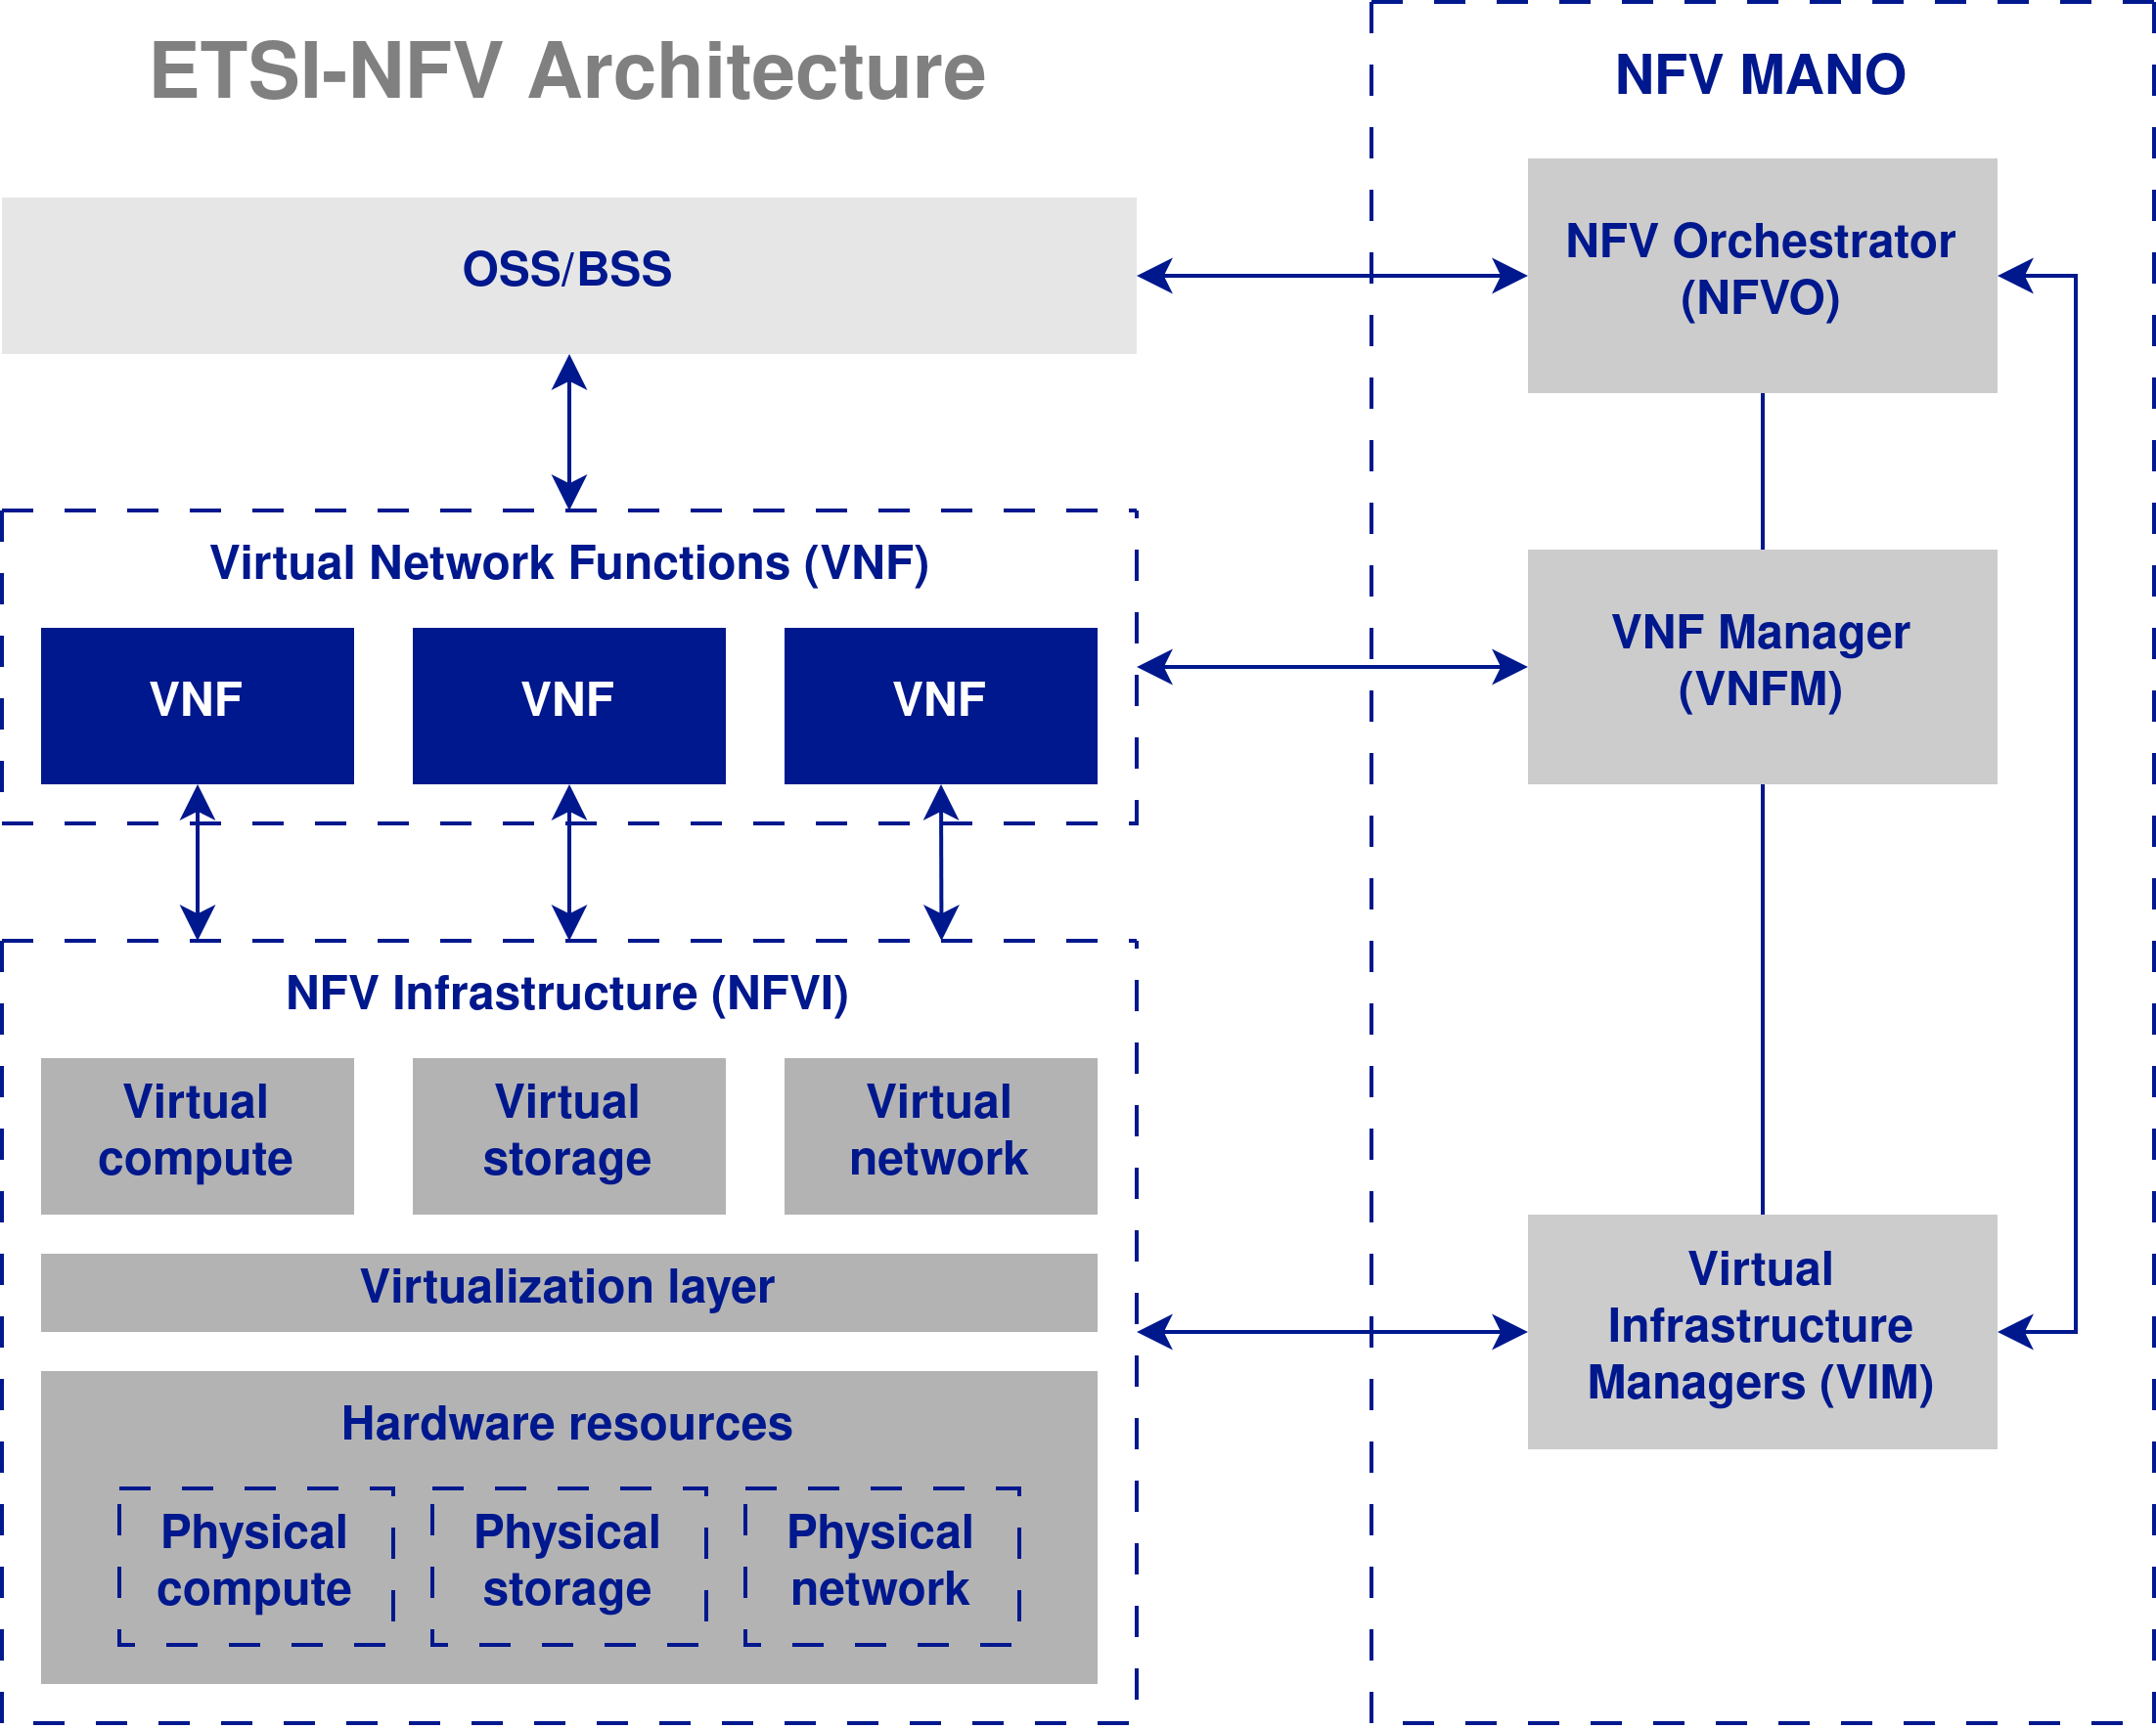
\includegraphics[width=0.8\linewidth]{figures/chapter1/nfv-architecture.png}
    \caption{ETSI NFV Architecture.}
    \label{fig:nfv_architecture}
\end{figure}

\subsubsection{Open Source MANO}

OSM\nomenclature{OSM}{Open Source MANO} \cite{Osm2026} is an open-source implementation of the NFV MANO framework, developed by ETSI, designed to be vendor-neutral and compliant with ETSI specifications. OSM provides a modular and extensible platform that supports the orchestration of both VNFs and CNFs across heterogeneous infrastructures, including VMs, containers, and hybrid environments. It integrates with multiple VIMs, such as OpenStack \cite{Openstack2026} and Kubernetes \cite{Kubernetes2026}, and offers support for multi-site and multi-domain deployments.

\section{Surveys on sustainable service orchestration strategies}

In recent years, Edge computing has emerged as a crucial paradigm for processing data closer to its source, significantly reducing latency and bandwidth usage. This paradigm shift necessitates advanced service orchestration techniques to efficiently manage and allocate resources across distributed Edge nodes. A key consideration in this context is the energy efficiency of these operations, as Edge devices often operate in resource-constrained environments where power consumption is a critical concern. Consequently, there is a growing focus on strategies to minimize energy consumption without compromising performance. In parallel, integrating renewable energy sources into Edge computing infrastructure has gained attention as a sustainable approach to reduce the carbon footprint of Edge services. This section is divided in three subsections to critically analyze existing studies and establish the research gap that motivates our work.

\subsection{Service orchestration for energy efficiency}

Existing literature on energy-efficient service orchestration can be categorized based on their scope and technical approach. However, a critical analysis reveals significant limitations in current approaches.

Several surveys focus exclusively on software-level optimizations while neglecting hardware-level energy management techniques. For instance, the authors in \cite{gaglianeseGreenOrchestrationCloudEdge2023} classify energy-aware approaches in the Cloud-Edge continuum but do not incorporate hardware management strategies such as DVFS or sleep mode operations. Similarly, the work presented in \cite{gitalEnergyManagementEdge2023} evaluates energy consumption metrics without addressing hardware-level optimizations and the survey in \cite{yangSurveyEnergyOptimization2023} focus only on task offloading and resource allocation strategies. Hardware management can contribute significantly to energy savings in Edge environments.

A portion of the literature addresses energy efficiency within specific application domains, limiting the generalization of findings. The authors of \cite{maoGreenEdgeAI2023} restrict their analysis to Edge AI applications, while in \cite{jiangEnergyefficientMechanismsSustainable2024} the focus is exclusively on Vehicular Fog Networks (VFN). The work in \cite{liuSurveyEdgeComputing2019} primarily studies existing Edge computing systems and open-source tools comparison. These domain-specific approaches, while valuable within their contexts, do not provide results applicable across diverse energy-efficient Edge computing scenarios.

Most critically, the majority of service orchestration studies operate under the assumption of traditional grid-powered infrastructure. The works in \cite{jiangEnergyAwareEdge2020} and \cite{congSurveyHierarchicalEnergy2020} address energy management and computation offloading without considering renewable energy integration. This represents a fundamental limitation because renewable energy alters orchestration strategies due to intermittency, varying power availability, energy storage constraints, and the need to manage multiple heterogeneous energy sources that traditional energy minimization approaches cannot adequately address.

\subsection{Renewable energy in Edge computing}

While renewable energy has gained attention in Edge computing research, current literature shows significant gaps in addressing its integration with service orchestration.

Several studies examine renewable energy in Edge computing contexts but fail to connect it with service orchestration strategies. The authors in \cite{israrRenewableEnergyPowered2021} explore renewable energy integration in 5G networks focusing on radio resource management, while the survey in \cite{rostirollaSurveyChallengesSolutions2022} provides extensive coverage of renewable energy in data centers but without Edge computing considerations. In \cite{pereraFogComputingSustainable2017}, the authors discuss Fog computing in smart cities but treat renewable energy and service orchestration as separate concerns. The work presented in \cite{sahRenewableEnergyHarvesting2020} addresses energy harvesting in wireless sensors without orchestration implications. These approaches do not study the synergies between renewable energy management and service orchestration.

When renewable energy is considered, it is typically constrained to specific use cases. The authors of \cite{guptaSurveyGreenUnmanned2022} limit their renewable energy discussion to solar power for roadside units and UAV applications, which may not translate to traditional Edge infrastructure scenarios.

A critical limitation in current literature is the predominant focus on energy harvesting for small-scale IoT devices rather than infrastructure-level renewable energy integration. The authors in \cite{shalaviEnergyEfficientDeployment2022} discuss energy-harvesting mobile Edge computing (EH-MEC) systems, but most cited works do not implement comprehensive renewable energy management. In \cite{benhamaidRecentAdvancesEnergy2022}, the authors concentrate on energy harvesting primarily for IoT devices, dividing discussions into energy harvesting and energy saving categories. This perspective overlooks crucial aspects of renewable energy integration including energy storage management, power prediction, grid interaction, and multi-source energy coordination that are essential for infrastructure-level implementations.

\subsection{Research gaps} \label{sec:research_gaps}

The critical analysis of existing literature reveals a fundamental research gap at the intersection of service orchestration and renewable energy integration in Edge computing. Current approaches have from three primary limitations:

\begin{itemize}
    \item Existing surveys typically address energy efficiency only in terms of reducing consumption during the orchestration process. The role and potential of renewable energy are often overlooked.
    \item In the few cases where renewable energy is considered, it is mainly viewed as a passive counterbalance to consumption. More advanced strategies, such as energy forecasting or the use of heterogeneous energy sources, are rarely explored in the service orchestration scenarios.
    \item Most renewable energy literature reviews in Edge computing focus on energy harvesting for IoT devices, while the orchestration strategies that integrate renewable energy at the infrastructure or data center level are largely neglected.
\end{itemize}

\section{Sustainability in service reconfiguration}

In dynamic environments characterized by variable renewable energy generation and potential node departures, service reconfiguration is essential to maintain system performance and sustainability. Two main categories of reconfiguration strategies can be identified in the context of sustainable orchestration. First, \emph{behavioral} reconfiguration strategies focus on adapting services by scaling, activating, or deactivating internal functions of deployed services based on current energy availability and workload demands. Second, \emph{structural} reconfiguration strategies involve modifying the placement of services across the infrastructure, migrating components to nodes with better energy profiles or lower risk of departure. While both strategies are essential, structural reconfiguration is particularly relevant in scenarios where node departures are unpredictable, as it allows for proactive adjustments to service placements to enhance robustness.

\subsection{Service Placement \& Placement reconfiguration}

Several works have addressed service placement in Cloud and Edge environments. In \cite{chenEnergyefficientServiceDeployment2024a}, the authors consider service deployment across Edge servers by accounting for geographical coordinates, user distribution patterns, and service preferences. In \cite{liangSustainableVirtualNetwork2024b}, the placement of VNFs in mobile Edge networks is studied, where VNFs are structured in service function chains (SFCs)\nomenclature{SFC}{Service Function Chain} for each user, and traffic must flow through the VNFs in sequence. In \cite{ahvarDECADynamicEnergy2021}, application components are distributed across different Edge clouds, and because components communicate with each other, placement decisions directly affect energy consumption. The authors of \cite{spinelliMigrationPathGreen2022} focus on job placement and migration in a MEC system, where each job is associated with revenue and cost. They show that migration decisions, while costly in terms of time and energy, can improve overall energy efficiency and QoS in contexts such as game session management. In \cite{fangResourceAllocationStrategy2020b}, VM migration is analyzed in the context of user mobility, with the goal of minimizing energy consumption as users move across the network. Similarly, container migration is studied in \cite{perinEASEEnergyAwareJob2023b}, where energy costs are considered, and migration decisions are only performed if they provide a net gain in energy efficiency. In \cite{guServiceManagementEnergy2023b}, the focus is on service management to reduce migration costs, while \cite{shenBackupBatteryAllocation2023} examines workload migration for balancing workload distribution, operational costs, and QoS trade-offs.

\subsection{Sustainability \& Robustness}

Only a small number of works explicitly consider renewable energy in this context. In \cite{liangSustainableVirtualNetwork2024b}, renewable energy (solar) is introduced in vehicular networks, while \cite{guServiceManagementEnergy2023b} explores solar and wind energy in Edge computing. Both models integrate batteries to store intermittent renewable energy. While several papers do account for renewable energy, such as \cite{guServiceManagementEnergy2023b,spinelliMigrationPathGreen2022,ahvarDECADynamicEnergy2021}, only \cite{haqueProvidingGreenSLAs2013} address it from a service-centered perspective. In that work, the concept of a green service level agreement (SLA)\nomenclature{SLA}{Service Level Agreement} is introduced, where services must consume at least a given percentage of energy from renewable sources. In addition to renewable energy, robustness to node departure is another important concern. Indeed, infrastructures in Edge computing are subject to various types of node departures, which can be voluntary, e.g. mobility, user-driven shutdowns, resource withdrawal, or non-voluntary, e.g. crash failures, connectivity loss, energy shortages, environmental hazards. To ensure service continuity, it is crucial to implement measures that mitigate the impact of these departures, especially when they cannot be predicted in advance. In \cite{yuMicroserviceResilienceDeployment2022}, a node diversity metric is proposed to evaluate microservice resilience to failures. The authors of \cite{chengResilientEdgeService2024} propose an uncertainty model for node failures in Edge computing. However, these approaches do not consider renewable energy, even though the intermittence of renewable sources and node departure risks are closely related.

\subsection{Prediction mechanisms}

Since renewable energy is intermittent, prediction mechanisms are necessary. Few works have addressed this problem. In \cite{perinEASEEnergyAwareJob2023b}, energy harvested from photovoltaic systems is estimated within a time window, with future power values modeled as Gaussian random variables. A receding horizon approach is then applied to solve scheduling decisions, allowing optimization of task execution based on expected energy availability. In \cite{haoEnergyAllocationTask2023c}, solar energy prediction is based on meteorological data, considering variables such as sunlight intensity, surface area, and conversion efficiency, with solar radiation as the main source of uncertainty. Similarly, \cite{angelajennifasujanaFogIntelligenceEnergy2024a} rely on meteorological data to forecast both light and power demand for solar-powered street lamps using quantile regression. In our contribution, we chose not to use meteorological data, as it might not always be available, and instead rely solely on historical power output and workload traces. We use a Sequence-to-Sequence (Seq2Seq) model \cite{sutskeverSequenceSequenceLearning2014} to predict both renewable energy generation and workload demands. Seq2Seq models have already been applied to energy-related forecasting tasks, such as energy consumption in industrial processes \cite{howindModelingEnergyConsumption2023} and day-ahead power generation scheduling in island power systems \cite{nishtarSeq2SeqBasedDayAheadSchedulingSCUC2024}.
  
\section{Practical implementation with NFV MANO} 

\subsection{NFV MANO Solutions}

\subsection{Cloud Platforms for NFV MANO}

\subsection{Energy-Aware NFV}

\section{Conclusion}

Our work is around three axes.

First, from gaps identified in Section \ref{sec:research_gaps}, we provide a new analysis of service orchestration strategies specifically designed for renewable energy-powered Edge computing environments. Unlike existing work that treats energy minimization and renewable energy as separate concerns, we examine orchestration strategies that explicitly account for renewable energy characteristics including intermittency, storage constraints and multi-source energy management. Our focus on orchestration strategies rather than optimization algorithms distinguishes this work from existing surveys that primarily consider algorithmic solutions. We analyze how renewable energy integration necessitates new orchestration strategies that go beyond traditional energy minimization by studying energy storage management, power prediction, renewable energy source coordination and grid interaction aspects that remain largely unexplored in current literature. This approach not only fills existing research voids but also provides a foundation for developing more sustainable and efficient Edge computing environments that can effectively use renewable energy sources through intelligent service orchestration.

Our second contribution addresses the problem of service placement and service placement reconfiguration. Unlike most existing works, which rely on battery-dependent systems, we focus on a battery-free infrastructure, an on-spot energy strategy, since batteries introduce high operational costs and require frequent replacement. In out scenario, all nodes are connected to the power grid, eliminating the need for batteries. Additionally, we integrate both sustainability and robustness as key optimization objectives, an approach that remains unexplored despite their complementary nature in renewable energy-enabled Edge systems. To further enhance our placement and placement reconfiguration algorithms, we employ a Seq2Seq model to forecast renewable energy generation and workload demand, enabling us to optimize our selected metrics more effectively.

\ifdefined\included
\else
\bibliographystyle{acm}
\bibliography{These}
\end{document}
\fi
